\section{Theoretical Setting}

\begin{frame}{The Underlying Model}
    \begin{block}{Setting 1: Data Generating Process}
        Let $T \in \mathbb{R}_{>0}$ be a fixed time horizon and $d \in \mathbb{N}$. We consider the relationship:
        \begin{equation}
            Y_t = X_t^\top \beta + U_t + \eta_t, \quad t \in [0,T]
        \end{equation}
    \end{block}
    {\small \textbf{Components:}
    \begin{itemize}
        \item \textbf{$X_t \in \mathbb{R}^d$}: a (multivariate) stochastic process.
        \item \textbf{$U_t \in \mathbb{R}$}: a (univariate) stochastic process.
        \item \textbf{$\eta_t$}: i.i.d. centered Gaussian noise independent of $X$.
        \item \textbf{$\beta \in \mathbb{R}^d$}: True causal effect (estimand).
    \end{itemize}
    \textbf{Observations:}
    Given a fixed $n \in \mathbb{N},$ we assume that we observe with $\Delta t = T/n$:
    \begin{itemize}
        \item $X^n := (X_{\Delta t}, X_{2\Delta t}, ..., X_{n\Delta t})^\top$
        \item $Y^n := (Y_{\Delta t}, Y_{2 \Delta t}, ..., Y_{n \Delta t})^\top$
    \end{itemize}}

    \textbf{In short:} $X^n$ and $Y^n$ are vectors of discrete (equidistant) $n$ observations, $U_t$ is a hidden confounder.
\end{frame}

\begin{frame}{Frequency Domain Transformation}
    \textbf{Recall:}
    Only discrete $X^n := (X_{\Delta t}, X_{2\Delta t}, ..., X_{n\Delta t})$ in time domain is given, not the continuous $X_t$ with $t \in [0, T]$
    \begin{block}{Basis Expansions}
        Given only $X^n$ ($n$ discrete observations), "reconstruct" the original process $X_t$ as a linear combination of basis functions:
        \begin{equation}
            \hat X_{i \Delta t} = \sum_{k = 1}^{K}\hat c_k \cdot \phi_k(i\Delta t)
        \end{equation}
    \end{block}
    \begin{itemize}
        \item We use same basis functions to "reconstruct" $Y^n$ (and $U^n$)
        \item Here, we will mainly use the (ordered) \textbf{orthonormal} cosine basis.
    \end{itemize}
\end{frame}

\begin{frame}{Frequency Domain Transformation - 1D Example}
        \begin{figure}
        \centering
        \includegraphics[width=\textwidth]{figures/theoretical_setting/frequency_domain_transformation_example.png}
        \caption{\small{Given the discrete sample points in time domain, continuous $X_t$ is "reconstructed" by fitting the coefficients of the basis functions.}}
    \end{figure}
\end{frame}

\begin{frame}{Frequency Domain Transformation (Cosine Basis)}
    \begin{figure}
        \centering
        
        \begin{subfigure}{0.5\textwidth}
            \centering
            % I removed the 0.9 scale since they have a whole slide now!
            \includegraphics[width=\linewidth]{figures/theoretical_setting/continuous_cosine_basis_functions.png}
        \end{subfigure}%
        \hfill
        \begin{subfigure}{0.5\textwidth}
            \centering
            \includegraphics[width=\linewidth]{figures/theoretical_setting/orthogonality_cosine_basis_functions.png}
        
        \end{subfigure}
        
        % You now have room for a nice, descriptive overall caption
        \vspace{0.5cm} % Adds a little breathing room above the main caption
        \caption{\textbf{Left:} Cosine Basis Functions.\\ \textbf{Right:} Orthogonality of Cosine Basis Functions; Inner product between basis functions of different frequencies results in zero.}
    \end{figure}
\end{frame}

\begin{frame}{Frequency Domain Transformation (Cont.)}
    \begin{block}{Estimating coefficients $c$}
        let $\Phi$ be the $n \times K$ matrix with entries $\Phi_{i,k} = \phi_k(i\Delta t)$ and $K =$ number of basis functions. We want to estimate the vector of coefficients $c = (c_1, ..., c_K)$. We consider the sum of squared errors:
        \begin{equation}
            \text{SSE}_X = \sum_{i=1}^n (X_{i\Delta t} - \hat X_{i\Delta t}) = (X^n - \Phi c)^\top (X^n - \Phi c)
        \end{equation}
        The least squares solution gives $\hat c = (\Phi ^\top \Phi)^{-1}\Phi^\top X^n$. \\
        For \textbf{orthonormal} basis, it holds that $\Phi^\top \Phi \approx nI_K$, which gives $\hat c \approx \frac{1}{n}\Phi^\top X^n$.
    \end{block}
    {\small
    Above, we used:
    \vspace{-0.3cm}
    \begin{itemize}
        \item For orthonormal basis, it holds: $\int_0^T\phi_k(t)\phi_m(t)dt = \begin{cases}1 & \text{if } k=m \\0 & \text{if } k \ne m \end{cases}$
        \item For $k = m$: Sum approximation yields: $\frac{1}{n}\sum_{i=1}^{n}\phi_k(i\Delta t)^2 \approx 1$.
    \end{itemize}
    }
\end{frame}

\begin{frame}{Frequency Domain Transformation}
Previous derivation: $\hat c \approx \frac{1}{n}\Phi^\top X^n$.
    \begin{block}{Transformation $T_k^{\phi,n}$}
        Let $\mathcal{D}$ be the set of n $\mathbb{R}^d$-valued discrete samples of stochastic processes (see $X^n$) and $\mathcal{C}$ the set of random variables on $\mathbb{R}^d$. Let timestamp $\Delta t = T/n$.
        Define, for all $k \le n$, the function $T_k^{\phi,n} : \mathcal{D} \to \mathcal{C}$ by:
        $$T_k^{\phi,n}(V) := \begin{bmatrix} 
        \frac{1}{n} \sum_{i=1}^n (V_{i\Delta t})_1 \phi_k(i\Delta t) \\ 
        \vdots \\ 
        \frac{1}{n} \sum_{i=1}^n (V_{i\Delta t})_d \phi_k(i\Delta t) 
        \end{bmatrix}$$
    \end{block}
    \begin{itemize}
        \item \textbf{\textcolor{blue}{$k \leq n$:}} Integer indices (Frequencies) of (ordered) orthonormal basis functions $\leq$ n (\# data points)
        \item \textbf{\textcolor{blue}{DCT:}} for the cosine basis, this corresponds to Discrete Cosine Transform
    \end{itemize}
\end{frame}

\begin{frame}{Assumptions and Sparsity}
\begin{block}{Definition 1: $(\phi, G)$-sparse process}
        A process $U$ is $(\phi, G)$-sparse with respect to basis $\phi$ if for a set $G \subseteq \mathbb{N}$:
        $$ \langle U, \phi_k \rangle_{L^2} = \int_0^T U_t \phi_k(t) dt = 0 \quad \text{for all } k \notin G \text{ almost surely} $$
    \end{block}

    \begin{alertblock}{Assumption 1: Sparse Confounding }
        The set $G$ is "small," meaning the hidden confounder only affects a few basis components (frequencies).
    \end{alertblock}

    \textbf{Implication:}
    \begin{itemize}
        \item From before: $\int_0^T U_t \phi_k(t) dt \approx \frac{1}{n}\sum_{i=1}^n(U_{i\Delta t})\phi_k(i\Delta t) = T_k^{\phi,n}(U)$
        \item By transforming the data, we can isolate the ``clean'' frequencies $G^c$ where the confounder disappears.
    \end{itemize}
\end{frame}

\begin{frame}[fragile]{Example: Sparse $U$}
    \begin{lstlisting}[language=Python]
import numpy as np
import matplotlib.pyplot as plt
from scipy.fft import dct

n = 500
T = 1.0  # Time horizon
t = np.linspace(0, T, n, endpoint=False)

# some small frequency set
k1, k2 = 2, 5

U_time = 2.0 * np.cos(2 * np.pi * k1 * t / T) + 1.0 * np.cos(2 * np.pi * k2 * t / T)

U_freq = dct(U_time, type=2, norm='ortho')
k_indices = np.arange(len(U_freq)) 
magnitude = np.abs(U_freq) / (n / 2) # Normalize

# 'magnitude` is zero everywhere except 
# exactly at the integer indices k=2 and k=5
    \end{lstlisting}
\end{frame}

\begin{frame}{Example: Sparse $U$}
    \begin{figure}
        \centering
        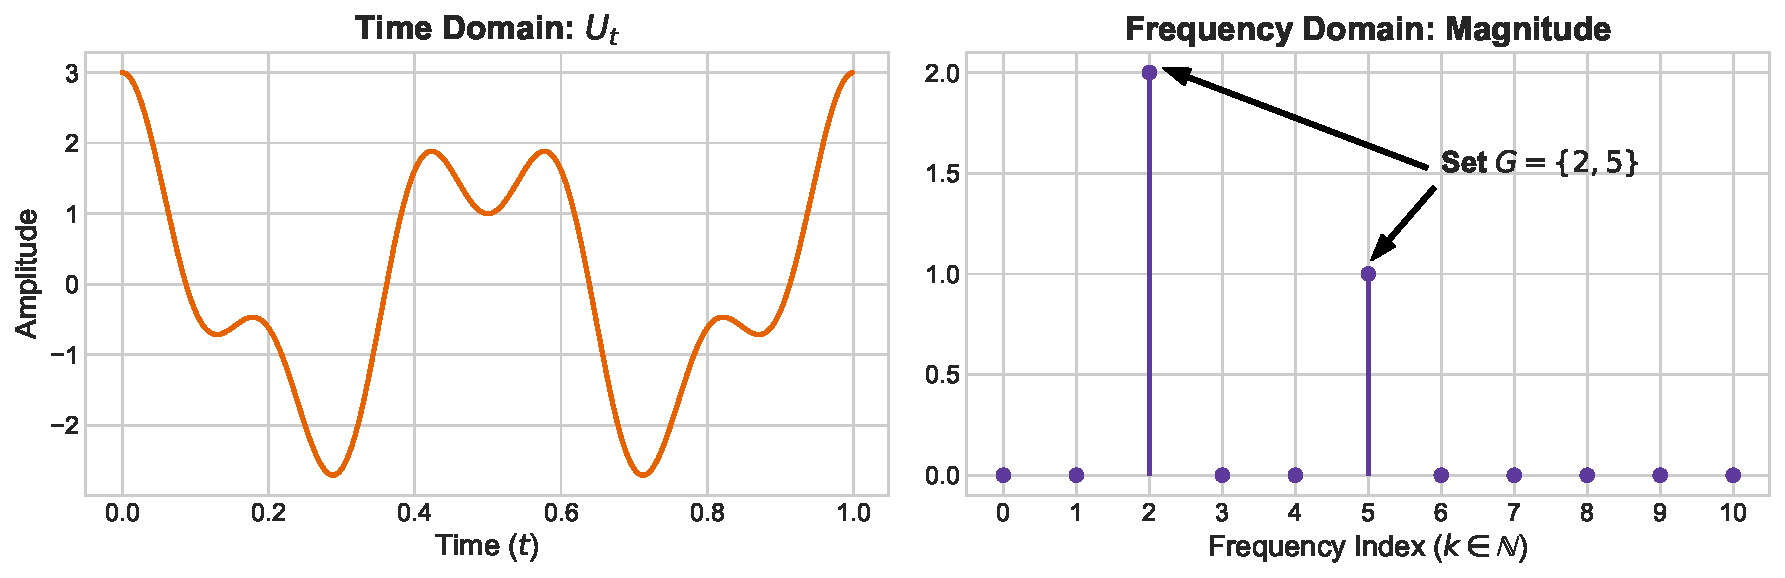
\includegraphics[width=\textwidth]{figures/theoretical_setting/sparse_U_example.pdf}
        \caption{A sparse confounder $U_t$ in the time domain (left) and frequency domain (right). The non-zero spikes represent the "small" confounded set $G$.}
    \end{figure}
\end{frame}



\begin{frame}{Frequency Domain Transformation - Outlier Problem}

    {\scriptsize from before:}
    {\small
    \[
    T_k^{\phi,n}(Y) =
    \begin{bmatrix}
    \frac{1}{n}\sum_{i=1}^n (Y_{i\Delta t})_1 \phi_k(i\Delta t)\\
    \vdots\\
    \frac{1}{n}\sum_{i=1}^n (Y_{i\Delta t})_d \phi_k(i\Delta t)
    \end{bmatrix}
    \qquad
    \text{and}\qquad
    Y_t = X_t^\top \beta + U_t + \eta_t,\; t\in[0,T].
    \]
    }
    \begin{block}{The Deconfounded View}
        Using the linearity of $T_k^{\phi,n}$, it holds for all $k \le n$:
        \begin{equation}
            \begin{aligned}
                T_k^{\phi,n}(Y) &= T_k^{\phi,n}(X)^\top \beta + T_k^{\phi,n}(U) + T_k^{\phi,n}(\eta) \\
                &\overset{\text{a.s.}}{=} \begin{cases} 
                T_k^{\phi,n}(X)^\top \beta + T_k^{\phi,n}(U) + T_k^{\phi,n}(\eta) & \text{if } k \in G, \\ 
                T_k^{\phi,n}(X)^\top \beta + T_k^{\phi,n}(\eta) & \text{if } k \notin G. 
                \end{cases}
            \end{aligned}
        \end{equation}
    \end{block}

    \begin{exampleblock}{Remark: The Outlier Problem}
        If $k \in G$, $T_k^{\phi,n}(U)$ acts as an \textbf{adversarial outlier}. If $k \notin G$, the confounder term is zero, leaving an unconfounded linear relationship.
    \end{exampleblock}
\end{frame}

\begin{frame}{Outlier Problem}
    \begin{figure}
        \centering
        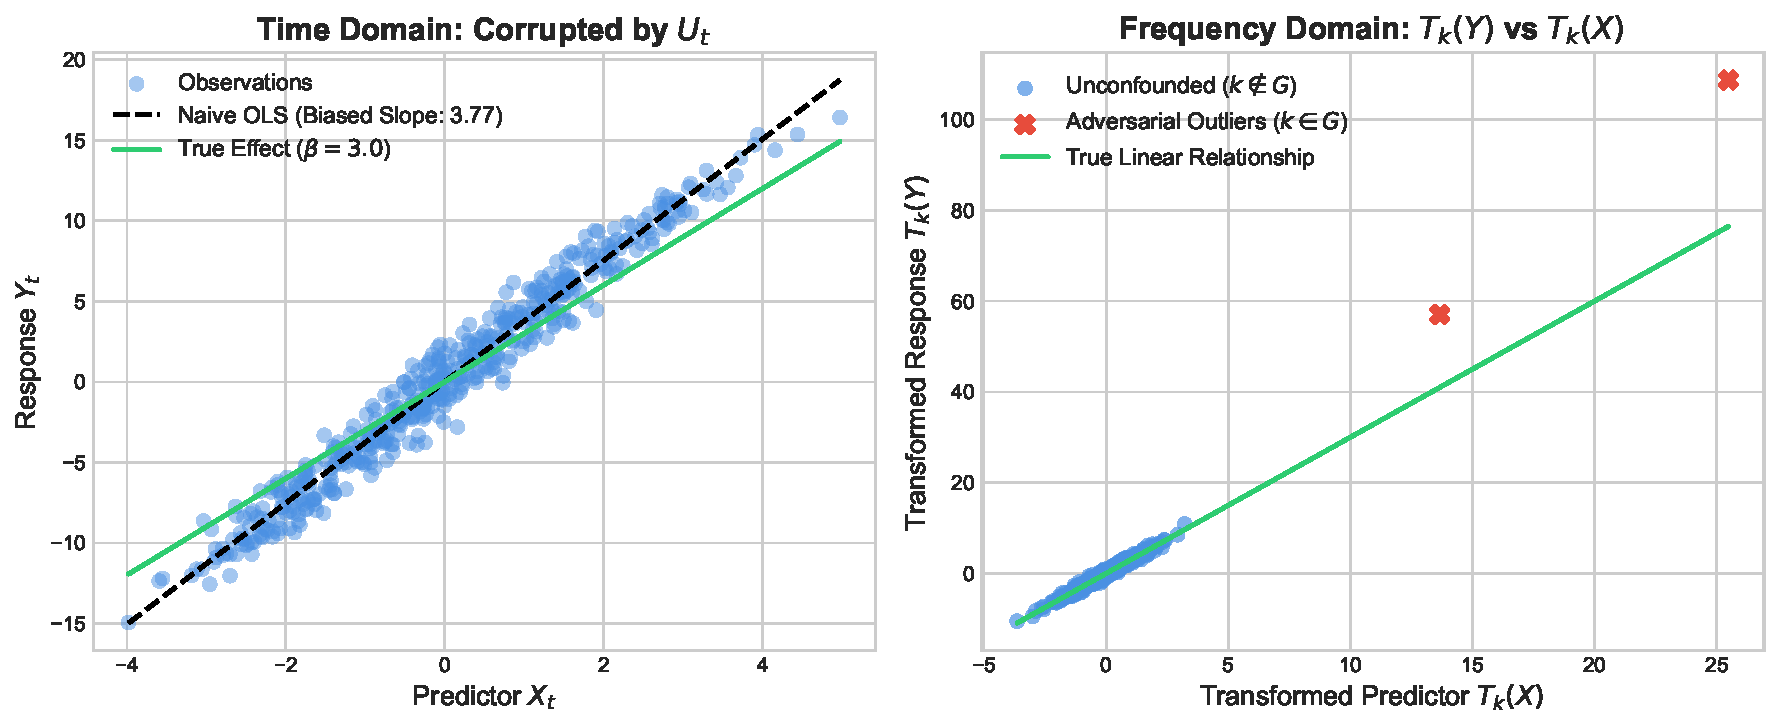
\includegraphics[width=\textwidth]{figures/theoretical_setting/outlier_problem_visualization.pdf}
        \caption{\textbf{Left:} In the time domain, the hidden confounder $U_t$ corrupts $X_t$ and the estimation of $\beta$ via OLS. \textbf{Right:} Applying DCT $T_k^{\phi,n}$ isolates the confounder into the sparse set $G$. The goal becomes identifying these isolated outliers and estimating the unconfounded relationship $\beta$ (via Robust Regression).}
    \end{figure}
\end{frame}